\documentclass[]{article}
\usepackage{lmodern}
\usepackage{amssymb,amsmath}
\usepackage{ifxetex,ifluatex}
\usepackage{fixltx2e} % provides \textsubscript
\ifnum 0\ifxetex 1\fi\ifluatex 1\fi=0 % if pdftex
  \usepackage[T1]{fontenc}
  \usepackage[utf8]{inputenc}
\else % if luatex or xelatex
  \ifxetex
    \usepackage{mathspec}
    \usepackage{xltxtra,xunicode}
  \else
    \usepackage{fontspec}
  \fi
  \defaultfontfeatures{Mapping=tex-text,Scale=MatchLowercase}
  \newcommand{\euro}{€}
\fi
% use upquote if available, for straight quotes in verbatim environments
\IfFileExists{upquote.sty}{\usepackage{upquote}}{}
% use microtype if available
\IfFileExists{microtype.sty}{%
\usepackage{microtype}
\UseMicrotypeSet[protrusion]{basicmath} % disable protrusion for tt fonts
}{}
\usepackage[margin=1in]{geometry}
\usepackage{color}
\usepackage{fancyvrb}
\newcommand{\VerbBar}{|}
\newcommand{\VERB}{\Verb[commandchars=\\\{\}]}
\DefineVerbatimEnvironment{Highlighting}{Verbatim}{commandchars=\\\{\}}
% Add ',fontsize=\small' for more characters per line
\usepackage{framed}
\definecolor{shadecolor}{RGB}{248,248,248}
\newenvironment{Shaded}{\begin{snugshade}}{\end{snugshade}}
\newcommand{\KeywordTok}[1]{\textcolor[rgb]{0.13,0.29,0.53}{\textbf{{#1}}}}
\newcommand{\DataTypeTok}[1]{\textcolor[rgb]{0.13,0.29,0.53}{{#1}}}
\newcommand{\DecValTok}[1]{\textcolor[rgb]{0.00,0.00,0.81}{{#1}}}
\newcommand{\BaseNTok}[1]{\textcolor[rgb]{0.00,0.00,0.81}{{#1}}}
\newcommand{\FloatTok}[1]{\textcolor[rgb]{0.00,0.00,0.81}{{#1}}}
\newcommand{\CharTok}[1]{\textcolor[rgb]{0.31,0.60,0.02}{{#1}}}
\newcommand{\StringTok}[1]{\textcolor[rgb]{0.31,0.60,0.02}{{#1}}}
\newcommand{\CommentTok}[1]{\textcolor[rgb]{0.56,0.35,0.01}{\textit{{#1}}}}
\newcommand{\OtherTok}[1]{\textcolor[rgb]{0.56,0.35,0.01}{{#1}}}
\newcommand{\AlertTok}[1]{\textcolor[rgb]{0.94,0.16,0.16}{{#1}}}
\newcommand{\FunctionTok}[1]{\textcolor[rgb]{0.00,0.00,0.00}{{#1}}}
\newcommand{\RegionMarkerTok}[1]{{#1}}
\newcommand{\ErrorTok}[1]{\textbf{{#1}}}
\newcommand{\NormalTok}[1]{{#1}}
\usepackage{longtable,booktabs}
\usepackage{graphicx}
\makeatletter
\def\maxwidth{\ifdim\Gin@nat@width>\linewidth\linewidth\else\Gin@nat@width\fi}
\def\maxheight{\ifdim\Gin@nat@height>\textheight\textheight\else\Gin@nat@height\fi}
\makeatother
% Scale images if necessary, so that they will not overflow the page
% margins by default, and it is still possible to overwrite the defaults
% using explicit options in \includegraphics[width, height, ...]{}
\setkeys{Gin}{width=\maxwidth,height=\maxheight,keepaspectratio}
\ifxetex
  \usepackage[setpagesize=false, % page size defined by xetex
              unicode=false, % unicode breaks when used with xetex
              xetex]{hyperref}
\else
  \usepackage[unicode=true]{hyperref}
\fi
\hypersetup{breaklinks=true,
            bookmarks=true,
            pdfauthor={Siyuan Meng; siyuanme@usc.edu},
            pdftitle={Data Mining for Diabetes Readmission Rate Prediction},
            colorlinks=true,
            citecolor=blue,
            urlcolor=blue,
            linkcolor=magenta,
            pdfborder={0 0 0}}
\urlstyle{same}  % don't use monospace font for urls
\setlength{\parindent}{0pt}
\setlength{\parskip}{6pt plus 2pt minus 1pt}
\setlength{\emergencystretch}{3em}  % prevent overfull lines
\setcounter{secnumdepth}{0}

%%% Use protect on footnotes to avoid problems with footnotes in titles
\let\rmarkdownfootnote\footnote%
\def\footnote{\protect\rmarkdownfootnote}

%%% Change title format to be more compact
\usepackage{titling}

% Create subtitle command for use in maketitle
\newcommand{\subtitle}[1]{
  \posttitle{
    \begin{center}\large#1\end{center}
    }
}

\setlength{\droptitle}{-2em}
  \title{Data Mining for Diabetes Readmission Rate Prediction}
  \pretitle{\vspace{\droptitle}\centering\huge}
  \posttitle{\par}
  \author{Siyuan Meng \\ \href{mailto:siyuanme@usc.edu}{\nolinkurl{siyuanme@usc.edu}}}
  \preauthor{\centering\large\emph}
  \postauthor{\par}
  \predate{\centering\large\emph}
  \postdate{\par}
  \date{December 8, 2015}



\begin{document}

\maketitle


\section{Project Homepage}\label{project-homepage}

The link of project repository is
\url{https://github.com/siyuan1992/EE660_Project}. For more information,
please see \texttt{README.md}.

\section{Abstract}\label{abstract}

The management of hyperglycemia in the hospitalized inpatient becomes
increasing recognized, due to the morbidity and mortality outcome
{[}1,2{]}. For most non-ICU (Inensive Care Unit) patients, anecdotal
evidence says that inpatient managenent is arbitrary and often leads to
either no treatment or wide fluctuations in glucose when traditional
management strategies are employed {[}3,4{]}. Thus, protocols are
recommended. Effective prediction on readmissions enables hospitals to
identify and target patients at high risk {[}5{]}. Therefore, the goals
are discovering major factors contributing to hospitals readmissions as
well as finding the effective method to predict the type of
readmissions. Top three most important features for prediction are
\texttt{Number of inpatient visits}, \texttt{Admission type} and
\texttt{Admission source}. The best method for classification is
boosting-tree classifier. However, with data pre-mining and QUEST
(Quick, Unbiased and Effecient Statistical Tree), there will be
5\%\textasciitilde{}7\% further accuray improvement.

\section{Problem Statement and Goals}\label{problem-statement-and-goals}

The data is from the Center for Clinical and Translational Research,
Viginia Commonwealth University, which presents 10 years (1999-2008) of
clinical care at 130 US hospitals and integrated delivery networks
{[}6{]}. The goals here are identify the major factors that contribute
to hospital readmissions as well as find the best model to predict the
readmission type given inpatient information.

The difficulties of this problem are mainly in the following aspects:

\begin{itemize}
\itemsep1pt\parskip0pt\parsep0pt
\item
  The dataset is relatively large (\textasciitilde{}100,000 samples, 49
  features)
\item
  Several features have large propotional missing data due to the fact
  that prior to the HITECH legislation of the American Reinvestment and
  Recovery Act in 2009 hospitals and clinics were not required to
  capture it in a structured format {[}6{]}.
\item
  Significant amounts of preprocessing required:

  \begin{itemize}
  \itemsep1pt\parskip0pt\parsep0pt
  \item
    The preliminary dataet contained multiple inpaitent visits for some
    patients and the observations could not be considered statistically
    independent {[}paper{]}.
  \item
    Even though the preliminary dataset was extracted from the database
    with processing, lots of redundant features still exist.
  \item
    Almost 80\% features are nominal. Thus, after feature encoding, data
    will be expanded into a large dimension, which makes feature
    selection and classification extremely time consuming.
  \item
    Class labels are hierarchical. Three types of readmission are
    \texttt{NO}, \texttt{\textgreater{}30}, \texttt{\textless{}30},
    i.e., whether a patient will have readmission and if the patient
    have, a hospitalization occurs within 30 days or not.
  \end{itemize}
\end{itemize}

\section{Literature Review}\label{literature-review}

The research artical {[}6{]} talked about the background information
about th dataset and the information of each feature, which as a
reference, helps me to deal with redundant features.

The other paper {[}5{]} analyze the influence of different features and
use some tricks to improve the performance. The trick they used are
listed here:

\begin{itemize}
\itemsep1pt\parskip0pt\parsep0pt
\item
  Data pre-mining

  \begin{itemize}
  \itemsep1pt\parskip0pt\parsep0pt
  \item
    Re-categorize readmission group from 3 groups to 2 groups
    (Readmission \textless{}30 days and Non-within 30 days.)
  \item
    Subsample to make readmission group's ratio be 1:1
  \item
    Review each feature's relationship with readmission
  \item
    Review numeric variables correlation
  \end{itemize}
\item
  Use QUEST model to improve accuracy.
\end{itemize}

Several gruops use the similar trick, like recategorizing readmission
groups to two (Readmission or not). However, data pre-mining is of
upmost importance in improving the model accuracy. With data pre-mining
and ensemble models, the highest accuracy could reach 80\% {[}7{]}.

\section{Prior and Related Work}\label{prior-and-related-work}

This project is exclusively for EE660.

\section{Project Formulation and
Setup}\label{project-formulation-and-setup}

I tried several modals and algorithms for this project, e.g.~Perceptron,
SVM, logistic classifier, etc. I want to list two of them which have
best performances.

\begin{itemize}
\itemsep1pt\parskip0pt\parsep0pt
\item
  The first is gradient tree boosting classifier. The algorithm
  (pseudocode) is as follows {[}8{]}:
\end{itemize}

\begin{longtable}[c]{@{}l@{}}
\toprule
\begin{minipage}[t]{0.97\columnwidth}\raggedright\strut
Input: training set \({(\textbf{x}_{i},y_{i})}_{i=1}^N\), loss function
\(L(y,f(\textbf{x}))\) and number of iteration M.
\strut\end{minipage}\tabularnewline
\begin{minipage}[t]{0.97\columnwidth}\raggedright\strut
Algorithm:
\strut\end{minipage}\tabularnewline
\begin{minipage}[t]{0.97\columnwidth}\raggedright\strut
I. Initialize model with a constant value:
\strut\end{minipage}\tabularnewline
\begin{minipage}[t]{0.97\columnwidth}\raggedright\strut
\[f_{0}(x)=\mathop{\arg\min}\limits_{\gamma}\sum_{i=1}^NL(y_i,\gamma)\].
\strut\end{minipage}\tabularnewline
\begin{minipage}[t]{0.97\columnwidth}\raggedright\strut
II. for m=1 to M:
\strut\end{minipage}\tabularnewline
\begin{minipage}[t]{0.97\columnwidth}\raggedright\strut
1. Compute pesudo-residuals:
\[r_{im}=-[\frac{\partial{L(y_i,f(\textbf{x}_i))}}{\partial{f(\textbf{x}_i)}}]_{f(\textbf{x})=f_{m-1}(\textbf{x})} \qquad  for\ i=1,...,N\].
\strut\end{minipage}\tabularnewline
\begin{minipage}[t]{0.97\columnwidth}\raggedright\strut
2. Train with training set \({(\textbf{x}_i,r_{im})}_{i=1}^N\).
\strut\end{minipage}\tabularnewline
\begin{minipage}[t]{0.97\columnwidth}\raggedright\strut
3. Compute \(\gamma{_m}\) by solving:
\[\gamma{_m}=\mathop{\arg\min}\limits_{\gamma}\sum_{i=1}^NL(y_i,f_{m-1}(\textbf{x}_i)+\gamma{h_m(\textbf{x}_i)})\].
\strut\end{minipage}\tabularnewline
\begin{minipage}[t]{0.97\columnwidth}\raggedright\strut
4. Update the model:
\[f_m(\textbf{x})=f_{m-1}(\textbf{x})+\gamma{_m}h_m(\textbf{x})\]
\strut\end{minipage}\tabularnewline
\begin{minipage}[t]{0.97\columnwidth}\raggedright\strut
III. Output \(F_M(\textbf{x})\).
\strut\end{minipage}\tabularnewline
\bottomrule
\end{longtable}

Parameters need to tune here are iteration number \(M\), maximum depth
of a tree and step size to solve \(\gamma\). In general, boosting will
not cause overfitting since it is a maximum margin classifier, which is
fundamentally equivalent to SVM. However, boosting is a non-parametric,
non-linear and non-binary method, which will lead to better result.

\begin{itemize}
\itemsep1pt\parskip0pt\parsep0pt
\item
  The second method is neuralnet classifier.
\end{itemize}

There is no single formal definition of what an artificial neural
network is. Typically, a class of statistical models could be called
``neural'' if it possesses the following characteristics {[}9{]}:

\begin{verbatim}
+ Contains sets of adaptive weights. 
+ Capability of approximating non-linear functions of their inputs.
\end{verbatim}

Training a neural network essentially means selecting one model form set
of allowed models {[}wiki{]}. The general framework is:

\begin{verbatim}
+ Model representation
+ Feedforward and cost function
+ Backpropagation to compute the gradient for the cost function
+ Gradient checking (Optional)
+ Get learning parameters, output result
\end{verbatim}

Parameters need to tune are number of iteration, number of layers, model
parameters\ldots{}In general, neural network may cause overfitting and
the speed is pretty low. However, neural network is good for non-linear
classification, and that's the reason why it has better performance
here.

Since both two methods are computational complicated, the trick I used
here is to use \texttt{graphlab\_create} in python, which reads csv
files in SFrame and classification is much faster than other packages
and other programming languages. Thus, tuning parameters is not
time-consuming. Also, due to the size of the dataset and the computation
complexity, using validation set randomly generated from training set
instead of using cross validation, though cross validation may lead to
better accuracy.

\section{Methodology}\label{methodology}

Here is my whole precedure for this project:

\begin{enumerate}
\def\labelenumi{\arabic{enumi}.}
\itemsep1pt\parskip0pt\parsep0pt
\item
  Download data online.
\item
  Set problem and goals.
\item
  Review revelant papers and online materials to have a better
  understand of data.
\item
  Preprocessing. This includes:

  \begin{itemize}
  \itemsep1pt\parskip0pt\parsep0pt
  \item
    Deal with missing values.
  \item
    Split the original data into training and test dataset with ratio
    8:2. (No need to generate validation set here, since the classifier
    will directly use part of training dataset as validation.)
  \item
    Subsample data. Considered only the first encounter for each patient
    as the primary admission and determined whether or not they were
    readmitted within 30 days. (Could do before splitting)
  \item
    Remove irrelevant features and near-zero features (variables) for
    both training and test dataset.
  \item
    Plot the histgram of class labels of training dataset. This is a
    imbalanced problem, so subsample training set to let different
    classes have same ratios. (Here, could try both over-sampling and
    under-sampling or give weights for different classes as a parameter
    to classifiers.)
  \item
    Convert catogegorical features to numerical for both training and
    test dataset.
  \item
    Feature dimension reduction for both training and test dataset.
  \item
    Feature normalization.
  \end{itemize}
\item
  Training and testing. This includes:

  \begin{itemize}
  \itemsep1pt\parskip0pt\parsep0pt
  \item
    Set hypothesis set first. (For different model, the hypothesis sets
    are different.)
  \item
    A learning algorithm is used on training dataset.
  \item
    Couldn't choose the best hypothesis based only on training set,
    since this may cause overfitting. Instead, using validation set to
    choose the best hypothesis.
  \item
    For different model, there will be different ``best'' hypothesis.
    Choose the best one based on the horizontal comparison.
  \item
    Testing on test dataset.
  \end{itemize}
\item
  Result interpretation.
\end{enumerate}

\section{Implementation}\label{implementation}

\begin{itemize}
\itemsep1pt\parskip0pt\parsep0pt
\item
  Reproducibility In order to get the same results, need certain set of
  packages, as well as setting a pseudo-random seed equal the one I
  used. The following libraries were used for this project in R:
\end{itemize}

\begin{Shaded}
\begin{Highlighting}[]
\KeywordTok{library}\NormalTok{(caret)}
\KeywordTok{library}\NormalTok{(randomForest)}
\KeywordTok{library}\NormalTok{(pander)}
\KeywordTok{library}\NormalTok{(psych)}
\KeywordTok{library}\NormalTok{(FactoMineR)}
\KeywordTok{library}\NormalTok{(ggplot2)}
\end{Highlighting}
\end{Shaded}

Here is the seed I set to generate pseudo-random numbers for spliting
training and test dataset. (see \texttt{Preprocessing} section)

\begin{Shaded}
\begin{Highlighting}[]
\KeywordTok{set.seed}\NormalTok{(}\DecValTok{12345}\NormalTok{)}
\end{Highlighting}
\end{Shaded}

\begin{itemize}
\itemsep1pt\parskip0pt\parsep0pt
\item
  Getting data
\end{itemize}

\begin{Shaded}
\begin{Highlighting}[]
\KeywordTok{setwd}\NormalTok{(}\StringTok{"~/Documents/2015Fall/EE660/EE660_Project"}\NormalTok{)}
\NormalTok{data <-}\StringTok{ }\KeywordTok{read.csv}\NormalTok{(}\StringTok{"~/Documents/2015Fall/EE660/EE660_Project/diabetic_data.csv"}\NormalTok{,}
                 \DataTypeTok{stringsAsFactors=}\NormalTok{T,}\DataTypeTok{na.strings =} \StringTok{'?'}\NormalTok{)}
\end{Highlighting}
\end{Shaded}

\begin{itemize}
\item
  Feature space The preliminary dataset has 101766 samples and 49
  features. The original feature could be found in
  \url{http://www.hindawi.com/journals/bmri/2014/781670/tab1/}. Here,
  just talk about some important features.

  \begin{itemize}
  \itemsep1pt\parskip0pt\parsep0pt
  \item
    \texttt{Race}, \texttt{Gender} and \texttt{Age} nominal features for
    a patient.
  \item
    \texttt{Admission type}, \texttt{Discharge disposition} and
    \texttt{Admission source} are nominal features, which describes the
    hospitalization condition. In the preliminary dataset, these three
    features are given as integer identifier. The mappings are as
    follows.
  \end{itemize}

  \begin{longtable}[c]{@{}cc@{}}
  \toprule
  \begin{minipage}[b]{0.26\columnwidth}\centering\strut
  admission\_type\_id
  \strut\end{minipage} &
  \begin{minipage}[b]{0.17\columnwidth}\centering\strut
  description
  \strut\end{minipage}\tabularnewline
  \midrule
  \endhead
  \begin{minipage}[t]{0.26\columnwidth}\centering\strut
  1
  \strut\end{minipage} &
  \begin{minipage}[t]{0.17\columnwidth}\centering\strut
  Emergency
  \strut\end{minipage}\tabularnewline
  \begin{minipage}[t]{0.26\columnwidth}\centering\strut
  2
  \strut\end{minipage} &
  \begin{minipage}[t]{0.17\columnwidth}\centering\strut
  Urgent
  \strut\end{minipage}\tabularnewline
  \begin{minipage}[t]{0.26\columnwidth}\centering\strut
  3
  \strut\end{minipage} &
  \begin{minipage}[t]{0.17\columnwidth}\centering\strut
  Elective
  \strut\end{minipage}\tabularnewline
  \begin{minipage}[t]{0.26\columnwidth}\centering\strut
  4
  \strut\end{minipage} &
  \begin{minipage}[t]{0.17\columnwidth}\centering\strut
  Newborn
  \strut\end{minipage}\tabularnewline
  \begin{minipage}[t]{0.26\columnwidth}\centering\strut
  5
  \strut\end{minipage} &
  \begin{minipage}[t]{0.17\columnwidth}\centering\strut
  Not Available
  \strut\end{minipage}\tabularnewline
  \begin{minipage}[t]{0.26\columnwidth}\centering\strut
  6
  \strut\end{minipage} &
  \begin{minipage}[t]{0.17\columnwidth}\centering\strut
  NULL
  \strut\end{minipage}\tabularnewline
  \begin{minipage}[t]{0.26\columnwidth}\centering\strut
  7
  \strut\end{minipage} &
  \begin{minipage}[t]{0.17\columnwidth}\centering\strut
  Trauma Center
  \strut\end{minipage}\tabularnewline
  \begin{minipage}[t]{0.26\columnwidth}\centering\strut
  8
  \strut\end{minipage} &
  \begin{minipage}[t]{0.17\columnwidth}\centering\strut
  Not Mapped
  \strut\end{minipage}\tabularnewline
  \bottomrule
  \end{longtable}

  \begin{longtable}[c]{@{}cc@{}}
  \toprule
  \begin{minipage}[b]{0.35\columnwidth}\centering\strut
  discharge\_disposition\_id
  \strut\end{minipage} &
  \begin{minipage}[b]{0.41\columnwidth}\centering\strut
  description
  \strut\end{minipage}\tabularnewline
  \midrule
  \endhead
  \begin{minipage}[t]{0.35\columnwidth}\centering\strut
  1
  \strut\end{minipage} &
  \begin{minipage}[t]{0.41\columnwidth}\centering\strut
  Discharged to home
  \strut\end{minipage}\tabularnewline
  \begin{minipage}[t]{0.35\columnwidth}\centering\strut
  2
  \strut\end{minipage} &
  \begin{minipage}[t]{0.41\columnwidth}\centering\strut
  Discharged/transferred to another short term hospital
  \strut\end{minipage}\tabularnewline
  \begin{minipage}[t]{0.35\columnwidth}\centering\strut
  3
  \strut\end{minipage} &
  \begin{minipage}[t]{0.41\columnwidth}\centering\strut
  Discharged/transferred to SNF
  \strut\end{minipage}\tabularnewline
  \begin{minipage}[t]{0.35\columnwidth}\centering\strut
  4
  \strut\end{minipage} &
  \begin{minipage}[t]{0.41\columnwidth}\centering\strut
  Discharged/transferred to ICF
  \strut\end{minipage}\tabularnewline
  \begin{minipage}[t]{0.35\columnwidth}\centering\strut
  5
  \strut\end{minipage} &
  \begin{minipage}[t]{0.41\columnwidth}\centering\strut
  Discharged/transferred to another type of inpatient care institution
  \strut\end{minipage}\tabularnewline
  \begin{minipage}[t]{0.35\columnwidth}\centering\strut
  6
  \strut\end{minipage} &
  \begin{minipage}[t]{0.41\columnwidth}\centering\strut
  Discharged/transferred to home with home health service
  \strut\end{minipage}\tabularnewline
  \begin{minipage}[t]{0.35\columnwidth}\centering\strut
  7
  \strut\end{minipage} &
  \begin{minipage}[t]{0.41\columnwidth}\centering\strut
  Left AMA
  \strut\end{minipage}\tabularnewline
  \begin{minipage}[t]{0.35\columnwidth}\centering\strut
  8
  \strut\end{minipage} &
  \begin{minipage}[t]{0.41\columnwidth}\centering\strut
  Discharged/transferred to home under care of Home IV provider
  \strut\end{minipage}\tabularnewline
  \begin{minipage}[t]{0.35\columnwidth}\centering\strut
  9
  \strut\end{minipage} &
  \begin{minipage}[t]{0.41\columnwidth}\centering\strut
  Admitted as an inpatient to this hospital
  \strut\end{minipage}\tabularnewline
  \begin{minipage}[t]{0.35\columnwidth}\centering\strut
  10
  \strut\end{minipage} &
  \begin{minipage}[t]{0.41\columnwidth}\centering\strut
  Neonate discharged to another hospital for neonatal aftercare
  \strut\end{minipage}\tabularnewline
  \begin{minipage}[t]{0.35\columnwidth}\centering\strut
  11
  \strut\end{minipage} &
  \begin{minipage}[t]{0.41\columnwidth}\centering\strut
  Expired
  \strut\end{minipage}\tabularnewline
  \begin{minipage}[t]{0.35\columnwidth}\centering\strut
  12
  \strut\end{minipage} &
  \begin{minipage}[t]{0.41\columnwidth}\centering\strut
  Still patient or expected to return for outpatient services
  \strut\end{minipage}\tabularnewline
  \begin{minipage}[t]{0.35\columnwidth}\centering\strut
  13
  \strut\end{minipage} &
  \begin{minipage}[t]{0.41\columnwidth}\centering\strut
  Hospice / home
  \strut\end{minipage}\tabularnewline
  \begin{minipage}[t]{0.35\columnwidth}\centering\strut
  14
  \strut\end{minipage} &
  \begin{minipage}[t]{0.41\columnwidth}\centering\strut
  Hospice / medical facility
  \strut\end{minipage}\tabularnewline
  \begin{minipage}[t]{0.35\columnwidth}\centering\strut
  15
  \strut\end{minipage} &
  \begin{minipage}[t]{0.41\columnwidth}\centering\strut
  Discharged/transferred within this institution to Medicare approved
  swing bed
  \strut\end{minipage}\tabularnewline
  \begin{minipage}[t]{0.35\columnwidth}\centering\strut
  16
  \strut\end{minipage} &
  \begin{minipage}[t]{0.41\columnwidth}\centering\strut
  Discharged/transferred/referred another institution for outpatient
  services
  \strut\end{minipage}\tabularnewline
  \begin{minipage}[t]{0.35\columnwidth}\centering\strut
  17
  \strut\end{minipage} &
  \begin{minipage}[t]{0.41\columnwidth}\centering\strut
  Discharged/transferred/referred to this institution for outpatient
  services
  \strut\end{minipage}\tabularnewline
  \begin{minipage}[t]{0.35\columnwidth}\centering\strut
  18
  \strut\end{minipage} &
  \begin{minipage}[t]{0.41\columnwidth}\centering\strut
  NULL
  \strut\end{minipage}\tabularnewline
  \begin{minipage}[t]{0.35\columnwidth}\centering\strut
  19
  \strut\end{minipage} &
  \begin{minipage}[t]{0.41\columnwidth}\centering\strut
  Expired at home. Medicaid only, hospice.
  \strut\end{minipage}\tabularnewline
  \begin{minipage}[t]{0.35\columnwidth}\centering\strut
  20
  \strut\end{minipage} &
  \begin{minipage}[t]{0.41\columnwidth}\centering\strut
  Expired in a medical facility. Medicaid only, hospice.
  \strut\end{minipage}\tabularnewline
  \begin{minipage}[t]{0.35\columnwidth}\centering\strut
  21
  \strut\end{minipage} &
  \begin{minipage}[t]{0.41\columnwidth}\centering\strut
  Expired, place unknown. Medicaid only, hospice.
  \strut\end{minipage}\tabularnewline
  \begin{minipage}[t]{0.35\columnwidth}\centering\strut
  22
  \strut\end{minipage} &
  \begin{minipage}[t]{0.41\columnwidth}\centering\strut
  Discharged/transferred to another rehab fac including rehab units of a
  hospital .
  \strut\end{minipage}\tabularnewline
  \begin{minipage}[t]{0.35\columnwidth}\centering\strut
  23
  \strut\end{minipage} &
  \begin{minipage}[t]{0.41\columnwidth}\centering\strut
  Discharged/transferred to a long term care hospital.
  \strut\end{minipage}\tabularnewline
  \begin{minipage}[t]{0.35\columnwidth}\centering\strut
  24
  \strut\end{minipage} &
  \begin{minipage}[t]{0.41\columnwidth}\centering\strut
  Discharged/transferred to a nursing facility certified under Medicaid
  but not certified under Medicare.
  \strut\end{minipage}\tabularnewline
  \begin{minipage}[t]{0.35\columnwidth}\centering\strut
  25
  \strut\end{minipage} &
  \begin{minipage}[t]{0.41\columnwidth}\centering\strut
  Not Mapped
  \strut\end{minipage}\tabularnewline
  \begin{minipage}[t]{0.35\columnwidth}\centering\strut
  26
  \strut\end{minipage} &
  \begin{minipage}[t]{0.41\columnwidth}\centering\strut
  Unknown/Invalid
  \strut\end{minipage}\tabularnewline
  \begin{minipage}[t]{0.35\columnwidth}\centering\strut
  30
  \strut\end{minipage} &
  \begin{minipage}[t]{0.41\columnwidth}\centering\strut
  Discharged/transferred to another Type of Health Care Institution not
  Defined Elsewhere
  \strut\end{minipage}\tabularnewline
  \begin{minipage}[t]{0.35\columnwidth}\centering\strut
  27
  \strut\end{minipage} &
  \begin{minipage}[t]{0.41\columnwidth}\centering\strut
  Discharged/transferred to a federal health care facility.
  \strut\end{minipage}\tabularnewline
  \begin{minipage}[t]{0.35\columnwidth}\centering\strut
  28
  \strut\end{minipage} &
  \begin{minipage}[t]{0.41\columnwidth}\centering\strut
  Discharged/transferred/referred to a psychiatric hospital of
  psychiatric distinct part unit of a hospital
  \strut\end{minipage}\tabularnewline
  \begin{minipage}[t]{0.35\columnwidth}\centering\strut
  29
  \strut\end{minipage} &
  \begin{minipage}[t]{0.41\columnwidth}\centering\strut
  Discharged/transferred to a Critical Access Hospital (CAH).
  \strut\end{minipage}\tabularnewline
  \bottomrule
  \end{longtable}

  \begin{longtable}[c]{@{}cc@{}}
  \toprule
  \begin{minipage}[b]{0.29\columnwidth}\centering\strut
  admission\_source\_id
  \strut\end{minipage} &
  \begin{minipage}[b]{0.37\columnwidth}\centering\strut
  description
  \strut\end{minipage}\tabularnewline
  \midrule
  \endhead
  \begin{minipage}[t]{0.29\columnwidth}\centering\strut
  1
  \strut\end{minipage} &
  \begin{minipage}[t]{0.37\columnwidth}\centering\strut
  Physician Referral
  \strut\end{minipage}\tabularnewline
  \begin{minipage}[t]{0.29\columnwidth}\centering\strut
  2
  \strut\end{minipage} &
  \begin{minipage}[t]{0.37\columnwidth}\centering\strut
  Clinic Referral
  \strut\end{minipage}\tabularnewline
  \begin{minipage}[t]{0.29\columnwidth}\centering\strut
  3
  \strut\end{minipage} &
  \begin{minipage}[t]{0.37\columnwidth}\centering\strut
  HMO Referral
  \strut\end{minipage}\tabularnewline
  \begin{minipage}[t]{0.29\columnwidth}\centering\strut
  4
  \strut\end{minipage} &
  \begin{minipage}[t]{0.37\columnwidth}\centering\strut
  Transfer from a hospital
  \strut\end{minipage}\tabularnewline
  \begin{minipage}[t]{0.29\columnwidth}\centering\strut
  5
  \strut\end{minipage} &
  \begin{minipage}[t]{0.37\columnwidth}\centering\strut
  Transfer from a Skilled Nursing Facility (SNF)
  \strut\end{minipage}\tabularnewline
  \begin{minipage}[t]{0.29\columnwidth}\centering\strut
  6
  \strut\end{minipage} &
  \begin{minipage}[t]{0.37\columnwidth}\centering\strut
  Transfer from another health care facility
  \strut\end{minipage}\tabularnewline
  \begin{minipage}[t]{0.29\columnwidth}\centering\strut
  7
  \strut\end{minipage} &
  \begin{minipage}[t]{0.37\columnwidth}\centering\strut
  Emergency Room
  \strut\end{minipage}\tabularnewline
  \begin{minipage}[t]{0.29\columnwidth}\centering\strut
  8
  \strut\end{minipage} &
  \begin{minipage}[t]{0.37\columnwidth}\centering\strut
  Court/Law Enforcement
  \strut\end{minipage}\tabularnewline
  \begin{minipage}[t]{0.29\columnwidth}\centering\strut
  9
  \strut\end{minipage} &
  \begin{minipage}[t]{0.37\columnwidth}\centering\strut
  Not Available
  \strut\end{minipage}\tabularnewline
  \begin{minipage}[t]{0.29\columnwidth}\centering\strut
  10
  \strut\end{minipage} &
  \begin{minipage}[t]{0.37\columnwidth}\centering\strut
  Transfer from critial access hospital
  \strut\end{minipage}\tabularnewline
  \begin{minipage}[t]{0.29\columnwidth}\centering\strut
  11
  \strut\end{minipage} &
  \begin{minipage}[t]{0.37\columnwidth}\centering\strut
  Normal Delivery
  \strut\end{minipage}\tabularnewline
  \begin{minipage}[t]{0.29\columnwidth}\centering\strut
  12
  \strut\end{minipage} &
  \begin{minipage}[t]{0.37\columnwidth}\centering\strut
  Premature Delivery
  \strut\end{minipage}\tabularnewline
  \begin{minipage}[t]{0.29\columnwidth}\centering\strut
  13
  \strut\end{minipage} &
  \begin{minipage}[t]{0.37\columnwidth}\centering\strut
  Sick Baby
  \strut\end{minipage}\tabularnewline
  \begin{minipage}[t]{0.29\columnwidth}\centering\strut
  14
  \strut\end{minipage} &
  \begin{minipage}[t]{0.37\columnwidth}\centering\strut
  Extramural Birth
  \strut\end{minipage}\tabularnewline
  \begin{minipage}[t]{0.29\columnwidth}\centering\strut
  15
  \strut\end{minipage} &
  \begin{minipage}[t]{0.37\columnwidth}\centering\strut
  Not Available
  \strut\end{minipage}\tabularnewline
  \begin{minipage}[t]{0.29\columnwidth}\centering\strut
  17
  \strut\end{minipage} &
  \begin{minipage}[t]{0.37\columnwidth}\centering\strut
  NULL
  \strut\end{minipage}\tabularnewline
  \begin{minipage}[t]{0.29\columnwidth}\centering\strut
  18
  \strut\end{minipage} &
  \begin{minipage}[t]{0.37\columnwidth}\centering\strut
  Transfer From Another Home Health Agency
  \strut\end{minipage}\tabularnewline
  \begin{minipage}[t]{0.29\columnwidth}\centering\strut
  19
  \strut\end{minipage} &
  \begin{minipage}[t]{0.37\columnwidth}\centering\strut
  Readmission to Same Home Health Agency
  \strut\end{minipage}\tabularnewline
  \begin{minipage}[t]{0.29\columnwidth}\centering\strut
  20
  \strut\end{minipage} &
  \begin{minipage}[t]{0.37\columnwidth}\centering\strut
  Not Mapped
  \strut\end{minipage}\tabularnewline
  \begin{minipage}[t]{0.29\columnwidth}\centering\strut
  21
  \strut\end{minipage} &
  \begin{minipage}[t]{0.37\columnwidth}\centering\strut
  Unknown/Invalid
  \strut\end{minipage}\tabularnewline
  \begin{minipage}[t]{0.29\columnwidth}\centering\strut
  22
  \strut\end{minipage} &
  \begin{minipage}[t]{0.37\columnwidth}\centering\strut
  Transfer from hospital inpt/same fac reslt in a sep claim
  \strut\end{minipage}\tabularnewline
  \begin{minipage}[t]{0.29\columnwidth}\centering\strut
  23
  \strut\end{minipage} &
  \begin{minipage}[t]{0.37\columnwidth}\centering\strut
  Born inside this hospital
  \strut\end{minipage}\tabularnewline
  \begin{minipage}[t]{0.29\columnwidth}\centering\strut
  24
  \strut\end{minipage} &
  \begin{minipage}[t]{0.37\columnwidth}\centering\strut
  Born outside this hospital
  \strut\end{minipage}\tabularnewline
  \begin{minipage}[t]{0.29\columnwidth}\centering\strut
  25
  \strut\end{minipage} &
  \begin{minipage}[t]{0.37\columnwidth}\centering\strut
  Transfer from Ambulatory Surgery Center
  \strut\end{minipage}\tabularnewline
  \begin{minipage}[t]{0.29\columnwidth}\centering\strut
  26
  \strut\end{minipage} &
  \begin{minipage}[t]{0.37\columnwidth}\centering\strut
  Transfer from Hospice
  \strut\end{minipage}\tabularnewline
  \bottomrule
  \end{longtable}

  \begin{itemize}
  \itemsep1pt\parskip0pt\parsep0pt
  \item
    Features with \texttt{Number of} are numerical features, which are
    records for encounters.
  \item
    \texttt{Diagnosis 1,2,3} are nominal features encoded in a
    hierarchical way.
  \item
    \texttt{Medical specialty} is an integer identifier of a specialty
    of the admitting physician, corresponding to 84 distinct values, for
    example, cardiology, internal medicine, family/general practice, and
    surgeon.
  \end{itemize}
\item
  Cleaning data
\end{itemize}

The original missing value information can be found in
\url{http://www.hindawi.com/journals/bmri/2014/781670/tab1/}. For
simplicity, only show features which have missing values.

\begin{longtable}[c]{@{}cccc@{}}
\toprule
\begin{minipage}[b]{0.20\columnwidth}\centering\strut
Feature\_name
\strut\end{minipage} &
\begin{minipage}[b]{0.09\columnwidth}\centering\strut
Type
\strut\end{minipage} &
\begin{minipage}[b]{0.35\columnwidth}\centering\strut
Discription
\strut\end{minipage} &
\begin{minipage}[b]{0.24\columnwidth}\centering\strut
Propotional\_missing
\strut\end{minipage}\tabularnewline
\midrule
\endhead
\begin{minipage}[t]{0.20\columnwidth}\centering\strut
Race
\strut\end{minipage} &
\begin{minipage}[t]{0.09\columnwidth}\centering\strut
Nominal
\strut\end{minipage} &
\begin{minipage}[t]{0.35\columnwidth}\centering\strut
Values: Caucasian, Asian, African American, Hispanic, and other
\strut\end{minipage} &
\begin{minipage}[t]{0.24\columnwidth}\centering\strut
2\%
\strut\end{minipage}\tabularnewline
\begin{minipage}[t]{0.20\columnwidth}\centering\strut
Weight
\strut\end{minipage} &
\begin{minipage}[t]{0.09\columnwidth}\centering\strut
Numeric
\strut\end{minipage} &
\begin{minipage}[t]{0.35\columnwidth}\centering\strut
Weight in pounds
\strut\end{minipage} &
\begin{minipage}[t]{0.24\columnwidth}\centering\strut
97\%
\strut\end{minipage}\tabularnewline
\begin{minipage}[t]{0.20\columnwidth}\centering\strut
Payer code
\strut\end{minipage} &
\begin{minipage}[t]{0.09\columnwidth}\centering\strut
Nominal
\strut\end{minipage} &
\begin{minipage}[t]{0.35\columnwidth}\centering\strut
Integer identifier corresponding to 23 distinct values, for example,
Blue Cross/Blue Shield, Medicare, and self-pay
\strut\end{minipage} &
\begin{minipage}[t]{0.24\columnwidth}\centering\strut
40\%
\strut\end{minipage}\tabularnewline
\begin{minipage}[t]{0.20\columnwidth}\centering\strut
Medical specialty
\strut\end{minipage} &
\begin{minipage}[t]{0.09\columnwidth}\centering\strut
Nominal
\strut\end{minipage} &
\begin{minipage}[t]{0.35\columnwidth}\centering\strut
Integer identifier of a specialty of the admitting physician,
corresponding to 84 distinct values
\strut\end{minipage} &
\begin{minipage}[t]{0.24\columnwidth}\centering\strut
50\%
\strut\end{minipage}\tabularnewline
\begin{minipage}[t]{0.20\columnwidth}\centering\strut
Diagnosis 3
\strut\end{minipage} &
\begin{minipage}[t]{0.09\columnwidth}\centering\strut
Nominal
\strut\end{minipage} &
\begin{minipage}[t]{0.35\columnwidth}\centering\strut
Additional secondary diagnosis (coded as first three digits of ICD9),
corresponding to 954 distinct values
\strut\end{minipage} &
\begin{minipage}[t]{0.24\columnwidth}\centering\strut
1\%
\strut\end{minipage}\tabularnewline
\bottomrule
\end{longtable}

The way I deal with missing values is to delete \texttt{Weight},
\texttt{Payer code} feaures (columns), since both features have more
than 50\% missing values and they are not relevant to classification.
However, \texttt{Medical speciality} was maintained, adding the value
``missing'' in order to account for missing values. {[}6{]}

\begin{Shaded}
\begin{Highlighting}[]
\NormalTok{data <-}\StringTok{ }\NormalTok{data[,}\KeywordTok{c}\NormalTok{(-}\DecValTok{6}\NormalTok{,-}\DecValTok{11}\NormalTok{)]}
\NormalTok{data$medical_specialty <-}\StringTok{ }\KeywordTok{factor}\NormalTok{(data$medical_specialty,}
                \DataTypeTok{levels=}\KeywordTok{c}\NormalTok{(}\KeywordTok{levels}\NormalTok{(data$medical_specialty),}\StringTok{'Missing'}\NormalTok{))}
\NormalTok{data[,}\DecValTok{10}\NormalTok{][}\KeywordTok{is.na}\NormalTok{(data$medical_specialty)] <-}\StringTok{ 'Missing'}
\NormalTok{data <-}\StringTok{ }\KeywordTok{na.omit}\NormalTok{(data)}
\KeywordTok{dim}\NormalTok{(data)}
\end{Highlighting}
\end{Shaded}

\begin{verbatim}
## [1] 98053    48
\end{verbatim}

In general, should split the original data into training and testing
first and then deal with the missing values. However, both methods will
yield same dimension of \texttt{data}. For simplicity, deal with NAs
first here.

\begin{itemize}
\item
  Preprocessing and Feature Extraction (Preprocessing is more crucial
  when using model based algorithms, e.g.~Linear Discrimant Analysis,
  Naive Bayes, Linear Regression\ldots{}than using non-parametrical
  algorithms.)

  \begin{itemize}
  \itemsep1pt\parskip0pt\parsep0pt
  \item
    There are also other ways to impute data, like knnimpute\ldots{}For
    convenience, try omitting NA rows first.
  \item
    The data has been preprocessed to ensure each encounter has a unique
    id. However, each patient may have more than one id.
  \end{itemize}

\begin{Shaded}
\begin{Highlighting}[]
\KeywordTok{length}\NormalTok{(}\KeywordTok{unique}\NormalTok{(data$encounter_id))}
\end{Highlighting}
\end{Shaded}

\begin{verbatim}
## [1] 98053
\end{verbatim}

\begin{Shaded}
\begin{Highlighting}[]
\KeywordTok{length}\NormalTok{(}\KeywordTok{unique}\NormalTok{(data$patient_nbr))}
\end{Highlighting}
\end{Shaded}

\begin{verbatim}
## [1] 68630
\end{verbatim}

  \begin{itemize}
  \itemsep1pt\parskip0pt\parsep0pt
  \item
    We thus used only one encounter per patient; in particular, we
    considered only the first encounter for each patient as the primary
    admission and determined whether or not they were readmitted within
    30 days. {[}6{]}
  \end{itemize}

\begin{Shaded}
\begin{Highlighting}[]
\NormalTok{data <-}\StringTok{ }\NormalTok{data[}\KeywordTok{order}\NormalTok{(data[,}\DecValTok{2}\NormalTok{]),]}
\NormalTok{unique_list <-}\StringTok{ }\KeywordTok{array}\NormalTok{(}\OtherTok{TRUE}\NormalTok{,}\KeywordTok{nrow}\NormalTok{(data))}
\NormalTok{for (l in }\DecValTok{2}\NormalTok{:}\KeywordTok{nrow}\NormalTok{(data))\{}
    \NormalTok{if (data[l,}\StringTok{'patient_nbr'}\NormalTok{]==data[l}\DecValTok{-1}\NormalTok{,}\StringTok{'patient_nbr'}\NormalTok{])\{}
        \NormalTok{unique_list[l]=}\OtherTok{FALSE}
    \NormalTok{\}}
\NormalTok{\}}
\NormalTok{data <-}\StringTok{ }\KeywordTok{subset}\NormalTok{(data,unique_list)}
\end{Highlighting}
\end{Shaded}

  \begin{itemize}
  \itemsep1pt\parskip0pt\parsep0pt
  \item
    Kill the first two features(\texttt{encounter\_id} and
    \texttt{patient\_nbr}) which are ids for encounted and patients.
    Besides, extract label column, which is the last column of
    \texttt{data}.
  \end{itemize}

\begin{Shaded}
\begin{Highlighting}[]
\NormalTok{data <-}\StringTok{ }\NormalTok{data[,}\KeywordTok{c}\NormalTok{(-}\DecValTok{1}\NormalTok{,-}\DecValTok{2}\NormalTok{)]}
\NormalTok{label <-}\StringTok{ }\NormalTok{data$readmitted}
\NormalTok{data <-}\StringTok{ }\NormalTok{data[,-}\DecValTok{46}\NormalTok{]}
\end{Highlighting}
\end{Shaded}

  \begin{itemize}
  \itemsep1pt\parskip0pt\parsep0pt
  \item
    Split this train data into training and test dataset according to
    the ratio 8:2 (set seed to make partioning reproducible).
  \end{itemize}

\begin{Shaded}
\begin{Highlighting}[]
\NormalTok{inTrain <-}\StringTok{ }\KeywordTok{createDataPartition}\NormalTok{(label,}\DataTypeTok{p=}\FloatTok{0.8}\NormalTok{,}\DataTypeTok{list=}\OtherTok{FALSE}\NormalTok{)}
\NormalTok{training <-}\StringTok{ }\NormalTok{data[inTrain,]}
\NormalTok{training_label <-}\StringTok{ }\NormalTok{label[inTrain]}
\NormalTok{test <-}\StringTok{ }\NormalTok{data[-inTrain,]}
\NormalTok{test_label <-}\StringTok{ }\NormalTok{label[-inTrain]}
\end{Highlighting}
\end{Shaded}

  \begin{itemize}
  \itemsep1pt\parskip0pt\parsep0pt
  \item
    Now, let's see if samples of different classes of \texttt{training}
    dataset are unbalanced.
  \end{itemize}

\begin{Shaded}
\begin{Highlighting}[]
\KeywordTok{par}\NormalTok{(}\DataTypeTok{cex=}\FloatTok{0.7}\NormalTok{,}\DataTypeTok{pin=}\KeywordTok{c}\NormalTok{(}\DecValTok{4}\NormalTok{,}\DecValTok{3}\NormalTok{))}
\KeywordTok{plot}\NormalTok{((training_label), }\DataTypeTok{xlab =} \StringTok{'Days to inpatient readmission'}\NormalTok{, }\DataTypeTok{ylab =} \StringTok{'frequency'}\NormalTok{,}
     \DataTypeTok{col =} \StringTok{'red'}\NormalTok{, }\DataTypeTok{main =} \StringTok{'Histogram of different classes'}\NormalTok{)}
\end{Highlighting}
\end{Shaded}

  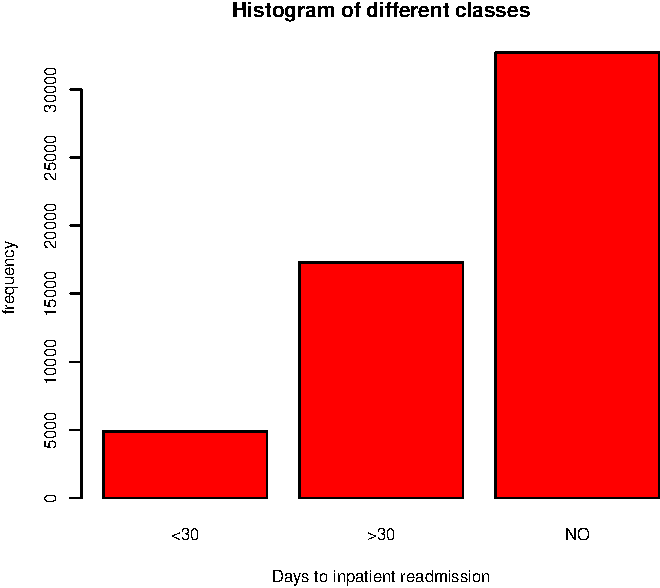
\includegraphics{Project_files/figure-latex/Preprocessing_classtype-1.pdf}

  \begin{itemize}
  \itemsep1pt\parskip0pt\parsep0pt
  \item
    Classes are unbalanced distributed in three levels, but not very
    skewed. Sampling data to deal with imbalanced classes, or to give
    weights in classifiers.
  \item
    Kill unimportant features.(\emph{nearZeroVar} diagnoses predictors
    that have one unique value (i.e.~are zero variance predictors) or
    predictors that are have both of the following characteristics: they
    have very few unique values relative to the number of samples and
    the ratio of the frequency of the most common value to the frequency
    of the second most common value is large.) {[}6{]}
  \end{itemize}

\begin{Shaded}
\begin{Highlighting}[]
\NormalTok{NZV <-}\StringTok{ }\KeywordTok{nearZeroVar}\NormalTok{(training,}\DataTypeTok{saveMetrics =} \NormalTok{T,}\DataTypeTok{freqCut=}\DecValTok{95}\NormalTok{/}\DecValTok{5}\NormalTok{)}
\NormalTok{training <-}\StringTok{ }\NormalTok{training[,-}\KeywordTok{which}\NormalTok{(NZV$nzv==}\OtherTok{TRUE}\NormalTok{)]}
\end{Highlighting}
\end{Shaded}

  \begin{itemize}
  \itemsep1pt\parskip0pt\parsep0pt
  \item
    Kill same features for \texttt{test} dataset without looking inside.
  \end{itemize}

\begin{Shaded}
\begin{Highlighting}[]
\NormalTok{test <-}\StringTok{ }\NormalTok{test[,-}\KeywordTok{which}\NormalTok{(NZV$nzv==}\OtherTok{TRUE}\NormalTok{)]}
\end{Highlighting}
\end{Shaded}

  \begin{itemize}
  \itemsep1pt\parskip0pt\parsep0pt
  \item
    Use background information for all features to analyze which
    features should be converted to numerical features.(Note: Need to
    combine training and test to a big dataset and then convert to
    numerical fearutes. If convert seperately, some feature may have
    some level which has only few points and are all assigned into
    \texttt{training} or \texttt{test} dataset. This may lead to
    different dimensions for \texttt{training} and \texttt{test} dataset
    after conversion.)
  \item
    First, drop large factors \texttt{diag2} and \texttt{diag3}.
  \end{itemize}

\begin{Shaded}
\begin{Highlighting}[]
    \NormalTok{training <-}\StringTok{ }\NormalTok{training[,}\KeywordTok{c}\NormalTok{(-}\DecValTok{16}\NormalTok{,-}\DecValTok{17}\NormalTok{)]}
    \NormalTok{test <-}\StringTok{ }\NormalTok{test[,}\KeywordTok{c}\NormalTok{(-}\DecValTok{16}\NormalTok{,-}\DecValTok{17}\NormalTok{)]}
\end{Highlighting}
\end{Shaded}

  \begin{itemize}
  \itemsep1pt\parskip0pt\parsep0pt
  \item
    Second, drop last nine features.
  \end{itemize}

\begin{Shaded}
\begin{Highlighting}[]
    \NormalTok{training <-}\StringTok{ }\NormalTok{training[,-}\KeywordTok{c}\NormalTok{(}\DecValTok{17}\NormalTok{:}\DecValTok{25}\NormalTok{)]}
    \NormalTok{test <-}\StringTok{ }\NormalTok{test[,-}\KeywordTok{c}\NormalTok{(}\DecValTok{17}\NormalTok{:}\DecValTok{25}\NormalTok{)]}
\end{Highlighting}
\end{Shaded}

  \begin{itemize}
  \itemsep1pt\parskip0pt\parsep0pt
  \item
    Third, convert categorical features to numerical features.
  \end{itemize}

\begin{Shaded}
\begin{Highlighting}[]
    \KeywordTok{source}\NormalTok{(}\StringTok{'~/Documents/2015Fall/EE660/EE660_Project/C2N.R'}\NormalTok{)}
    \NormalTok{data <-}\StringTok{ }\KeywordTok{rbind}\NormalTok{(training,test)}
    \NormalTok{for (i in }\KeywordTok{c}\NormalTok{(}\DecValTok{1}\NormalTok{:}\DecValTok{6}\NormalTok{,}\DecValTok{8}\NormalTok{,}\DecValTok{15}\NormalTok{))\{}
        \NormalTok{temp <-}\StringTok{ }\KeywordTok{as.factor}\NormalTok{(data[,i])}
        \NormalTok{data <-}\StringTok{ }\KeywordTok{cbind}\NormalTok{(data,}\KeywordTok{C2N}\NormalTok{(temp))}
    \NormalTok{\}}
    \NormalTok{data <-}\StringTok{ }\NormalTok{data[,-}\KeywordTok{c}\NormalTok{(}\DecValTok{1}\NormalTok{:}\DecValTok{6}\NormalTok{,}\DecValTok{8}\NormalTok{,}\DecValTok{15}\NormalTok{)]}
    \NormalTok{training <-}\StringTok{ }\NormalTok{data[}\DecValTok{1}\NormalTok{:}\KeywordTok{length}\NormalTok{(training_label),]}
    \NormalTok{test <-}\StringTok{ }\NormalTok{data[(}\KeywordTok{length}\NormalTok{(training_label)+}\DecValTok{1}\NormalTok{):}\DecValTok{68630}\NormalTok{,]}
\end{Highlighting}
\end{Shaded}

  \begin{itemize}
  \itemsep1pt\parskip0pt\parsep0pt
  \item
    Again, kill unimportant features using \emph{nearZeroVar}.
  \end{itemize}

\begin{Shaded}
\begin{Highlighting}[]
\NormalTok{NZV_2 <-}\StringTok{ }\KeywordTok{nearZeroVar}\NormalTok{(training,}\DataTypeTok{saveMetrics =} \NormalTok{T,}\DataTypeTok{freqCut=}\DecValTok{95}\NormalTok{/}\DecValTok{5}\NormalTok{)}
\NormalTok{training <-}\StringTok{ }\NormalTok{training[,-}\KeywordTok{which}\NormalTok{(NZV_2$nzv==}\OtherTok{TRUE}\NormalTok{)]}
\NormalTok{test<-}\StringTok{ }\NormalTok{test[,-}\KeywordTok{which}\NormalTok{(NZV_2$nzv==}\OtherTok{TRUE}\NormalTok{)]}
\end{Highlighting}
\end{Shaded}

  \begin{itemize}
  \itemsep1pt\parskip0pt\parsep0pt
  \item
    Normalize data (There are lots of differnt methods for
    normalization. However, this has the best performance.)
  \end{itemize}

\begin{Shaded}
\begin{Highlighting}[]
\NormalTok{training <-}\StringTok{ }\KeywordTok{apply}\NormalTok{(training,}\DecValTok{2}\NormalTok{,as.numeric)}
\NormalTok{test <-}\StringTok{ }\KeywordTok{apply}\NormalTok{(test,}\DecValTok{2}\NormalTok{,as.numeric)}
\NormalTok{training_std <-}\StringTok{ }\KeywordTok{apply}\NormalTok{(training,}\DecValTok{2}\NormalTok{,function(x) (x-}\KeywordTok{mean}\NormalTok{(x))/}\KeywordTok{sd}\NormalTok{(x))}
\NormalTok{test_std <-}\StringTok{ }\KeywordTok{apply}\NormalTok{(test,}\DecValTok{2}\NormalTok{,function(x) (x-}\KeywordTok{mean}\NormalTok{(x))/}\KeywordTok{sd}\NormalTok{(x))}
\end{Highlighting}
\end{Shaded}
\item
  Save \texttt{training} and \texttt{test} into csv file for future use.
\end{itemize}

\begin{Shaded}
\begin{Highlighting}[]
\KeywordTok{write.csv}\NormalTok{(}\KeywordTok{cbind}\NormalTok{(training_std,training_label),}\StringTok{'training.csv'}\NormalTok{,}\DataTypeTok{row.names =} \OtherTok{FALSE}\NormalTok{)}
\KeywordTok{write.csv}\NormalTok{(}\KeywordTok{cbind}\NormalTok{(test_std,test_label),}\StringTok{'test.csv'}\NormalTok{,}\DataTypeTok{row.names =} \OtherTok{FALSE}\NormalTok{)}
\end{Highlighting}
\end{Shaded}

Purpose for doing that is \texttt{R} is good for exploratory research,
but not good at dealing with large dataset for clasification. Use
\texttt{Python} to read csv as \texttt{SFrame} for classification will
speed up!

\begin{itemize}
\itemsep1pt\parskip0pt\parsep0pt
\item
  Training and testing are finished in python using
  \texttt{graphlab\_create}. Take \texttt{boosting tree classifier} as
  an example. The way I choose parameters are in a heuristics way. For
  example, the higher iteration number, the higher the accuracy for
  training dataset. However, accuracy will not increase any more at some
  iteration for validation set. Thus, choose that iteration number as
  the best parameter. Same way to choose other parameters. The best
  parameters I used in \texttt{boosting tree classifier} are:

  \begin{itemize}
  \itemsep1pt\parskip0pt\parsep0pt
  \item
    Number of iteration:30
  \item
    Maximum depth of tree:6
  \item
    Stepsize:0.3 Here, \texttt{boosting tree classifier} has the best
    performance.
  \end{itemize}
\end{itemize}

\section{Final results}\label{final-results}

The final accuracy using \texttt{boosting tree classifier} is around
70\% accuracy, which is the best among all models I used. Since randomly
assign class label will yield around 30\% accuracy, 70\% accuracy is a
huge improvement. There are lots of researches using this dataset for
classification. The best performance is around 70\%\textasciitilde{}80\%
accuracy{[}5,7{]}. However, the most importance factor for improving the
result is data pre-mining instead of choosing more advanced models.

\section{Summary and Conclusions}\label{summary-and-conclusions}

\begin{itemize}
\itemsep1pt\parskip0pt\parsep0pt
\item
  Data pre-mining is of upmost importance in improving the model
  accuracy, especially for this imbalanced-class problem.
\item
  Import factors for predicting readmission types are
  \texttt{admission source}, \texttt{admission type},
  \texttt{discharge disposition} and
  \texttt{number of inpatient visits}.
\item
  \texttt{Boosting tree classifier} is the most powerful classifier in
  this problem. In general, \texttt{boosting tree} a powerful tool in
  classification and regression.
\item
  Hospitals are advised to concern not only inpatient treatment but also
  continuing care after discharge since \texttt{\textless{}30} is the
  least frequent class.
\end{itemize}

\section{Reference}\label{reference}

\begin{enumerate}
\def\labelenumi{\arabic{enumi}.}
\itemsep1pt\parskip0pt\parsep0pt
\item
  G. E. Umpierrez, S. D. Isaacs, N. Bazargan, X. You, L. M. Thaler, and
  A. E. Kitabchi, ``Hyperglycemia: an independent marker of in-hospital
  mortality in patients with undiagnosed diabetes,'' Journal of Clinical
  Endocrinology and Metabolism, vol.~87, no. 3, pp.~978--982, 2002.
\item
  C. S. Levetan, M. Passaro, K. Jablonski, M. Kass, and R. E. Ratner,
  ``Unrecognized diabetes among hospitalized patients,'' Diabetes Care,
  vol.~21, no. 2, pp.~246--249, 1998.
\item
  A. G. Pittas, R. D. Siegel, and J. Lau, ``Insulin therapy for
  critically ill hospitalized patients: a meta-analysis of randomized
  controlled trials,'' Archives of Internal Medicine, vol.~164, no. 18,
  pp.~2005--2011, 2004.
\item
  A. C. Tricco, N. M. Ivers, J. M. Grimshaw et al., ``Effectiveness of
  quality improvement strategies on the management of diabetes: a
  systematic review and meta-analysis,'' The Lancet, vol.~379, no. 9833,
  pp.~2252--2261, 2012.
\item
  Data Mining for Diabetes Readmission Prediction Team Evolution Yi Chun
  Chien, Xiayu Zeng, Hong Zhang, Yixi Zhang
\item
  Strack, B., DeShazo, J. P., Gennings, C., et al.: Impact of HbA1c
  measurement on hospital readmission rates: Analysis of 70,000 clinical
  database patient records. Biomed. Res. Int., 2014, 2014, ID 781670.
\item
  \url{https://cepd.okstate.edu/files/11-Improving-the-Performance-of-two-stage-modeling.pdf}.
\item
  \url{https://en.wikipedia.org/wiki/Gradient_boosting}.
\item
  \url{https://en.wikipedia.org/wiki/Artificial_neural_network}.
\end{enumerate}

\end{document}
